\documentclass[10pt]{beamer}

\usetheme{simear}

\title{Implementing QVMP using QROM}
\author{Elton Pinto}
\date{\today}

\usepackage{algorithm}
\usepackage{algpseudocode}
\usepackage[braket, qm]{qcircuit}
\usepackage{subcaption}

\begin{document}

\begin{frame}[plain]
\titlepage
\end{frame}


% Outline

% Main contributions
% Grover search
  % Oracles - blackbox
  % Main difficulty is porting classical functions to quantum
    % What are the challenges?
  % Why is this useful to study?
  % Related: Amplitude Amplification
% QVMP
  % Algorithm - runtime and overview
  % Implementation details
    % QROM
    % Inner product
    % Circuit metrics
    % Transpilation times
% Future work
  % Automatic synthesis of Grover oracles from classical decision functions
    % Support for linear algebra operations
    % Integration with formal verification tooling
  % Investigate more efficient encodings of matrices and related operations
  % Investigate bottle-necks in transpilation
    % Cursory investigation revealed transpiler spends time performing SWAPs
    % which do not seem to be needed for fully connected qubit maps
  
\begin{frame}{Main contributions}
  \begin{itemize}
    \item Working implementation of QVMP in Qiskit
    \item Circuit metrics (gate count, circuit depth)
    \item Transpilation and simulation times
  \end{itemize}
\end{frame}

\begin{frame}{Motivation}
  \begin{itemize}
    \item Grover search: popular quantum search algorithm
    \item Depends on a black-box oracle to perform the search
    \item Offers quadratic speedup over classical linear search with a
      runtime of $O(\sqrt{N})$
    \item Related: Amplitude amplfication, a generalization of Grover search
  \end{itemize}
\end{frame}

\begin{frame}{Motivation (contd)}
  \begin{itemize}
    \item Core of Grover search straightforward to implement
    \item {
      Main challenge: encoding the oracle as a quantum circuit
      \begin{itemize}
        \item Debugging oracles is tricky due to non-determinism
        \item How to verify correctness?
      \end{itemize}
    }
  \end{itemize}

  \begin{alertblock}{Goal}
    Implement QVMP to better understand these challenges and investigate
    enhancements
  \end{alertblock}
\end{frame}

\begin{frame}{QVMP}
  \begin{itemize}
    \item Quantum Verification of Matrix Products
    \item Given $n \times n$ matrices $A$, $B$ and $C$, check if $AB = C$
    \item {
        Two quantum algorithms:
        \begin{itemize}
          \item Grover search based: $O(n^{\frac{7}{4}})$
          \item Quantum random walk based: $O(n^{\frac{5}{3}})$
        \end{itemize}
    }
  \end{itemize}
\end{frame}

\begin{frame}{QVMP Algorithm}
\begin{algorithm}[H]
  \caption{Quantum VMP using Grover Search}
  \label{alg:qvmp_grover}
  \textbf{Input: } $n \times n$ matrices $A, B, C$ \\
  \textbf{Output: } 1 if $AB = C$ and 0 otherwise \\
  \textbf{Procedure: }
  \begin{enumerate}
    \item Partition $B$ and $C$ into sub-matrices of size $n \times \sqrt{n}$
    \item 
      {
        Perform amplitude amplification for $n^{\frac{1}{4}}$ iterations using this subroutine:
        \begin{enumerate}
          \item Pick a random vector $x$ of size $\sqrt{n}$
          \item Classically compute $y = B_ix$ and $z = C_ix$
          \item Using Grover search with $\sqrt{n}$ iterations, find a row of
            index $j$ such that $(Ay \neq z)_j$
        \end{enumerate}
      }
    \item XOR the sub-results
  \end{enumerate}
\end{algorithm}
\end{frame}

\begin{frame}[fragile]{QVMP Implementation}
  \begin{lstlisting}[frame=single,language=Python, numbers=left]
# QVMP oracle described using a classical function

def find_row_mismatch(A, y, z):
  z_prime = A * y
  for j, value in enumerate(z_prime):
    if value != z[j]:
      return j
  return -1
  \end{lstlisting}

  \begin{itemize}
    \item The above snippet is encoded as a quantum circuit and constitutes
      the oracle
    \item QROM is used to efficiently encode the matrix
    \item Out-of-place inner product performs the row-vector multiplication
  \end{itemize}
\end{frame}

\begin{frame}{QROM - Quantum Read-only Memory}
  \begin{itemize}
    \item Encodes an $n \times m$ binary matrix using only $n + \log_2(n)$ qubits
    \item Outputs the value of the $j$th row indexed using address qubits
    \item Can use superposition to extract multiple rows
  \end{itemize}
  \begin{figure}
      \centering
      \scalebox{0.8}{
      \begin{minipage}{\textwidth}
          \begin{equation*}
            A = \begin{bmatrix}%
              0 & 1 & 0 & 1 \\
              1 & 1 & 1 & 0 \\
              1 & 0 & 0 & 1 \\
              1 & 0 & 1 & 0 \\
            \end{bmatrix}
          \end{equation*}
      \end{minipage}
      }
      \begin{subfigure}{\textwidth}
        \centering
        \scalebox{0.8}{
  \begin{minipage}{\textwidth}
    \begin{equation*}
      A = \begin{bmatrix}%
        0 & 1 & 0 & 1 \\
        1 & 1 & 1 & 0 \\
        1 & 0 & 0 & 1 \\
        1 & 0 & 1 & 0 \\
      \end{bmatrix}
    \end{equation*}
  \end{minipage}
}
\begin{subfigure}{\textwidth}
  \centering
  \scalebox{0.8}{
            \Qcircuit @C=1.0em @R=0.2em @!R { \\
  	      \nghost{{addr}_{0} :  } & \lstick{{addr}_{0} :  } & \gate{\mathrm{X}} & \ctrl{1} & \ctrl{1} \barrier[0em]{5} & \qw & \gate{\mathrm{X}} & \ctrl{1} & \ctrl{1} \barrier[0em]{5} & \qw & \qw & \ctrl{1} & \ctrl{1} \barrier[0em]{5} & \qw & \gate{\mathrm{X}} & \ctrl{1} & \ctrl{1} \barrier[0em]{5} & \qw & \qw & \qw\\
  	      \nghost{{addr}_{1} :  } & \lstick{{addr}_{1} :  } & \gate{\mathrm{X}} & \ctrl{2} & \ctrl{4} & \qw & \qw & \ctrl{1} & \ctrl{4} & \qw & \gate{\mathrm{X}} & \ctrl{1} & \ctrl{2} & \qw & \qw & \ctrl{1} & \ctrl{2} & \qw & \qw & \qw\\
  	      \nghost{{data}_{0} :  } & \lstick{{data}_{0} :  } & \qw & \qw & \qw & \qw & \qw & \targ & \qw & \qw & \qw & \targ & \qw & \qw & \qw & \targ & \qw & \qw & \qw & \qw\\
  	      \nghost{{data}_{1} :  } & \lstick{{data}_{1} :  } & \qw & \targ & \qw & \qw & \qw & \qw & \qw & \qw & \qw & \qw & \targ & \qw & \qw & \qw & \targ & \qw & \qw & \qw\\
  	      \nghost{{data}_{2} :  } & \lstick{{data}_{2} :  } & \qw & \qw & \qw & \qw & \qw & \qw & \qw & \qw & \qw & \qw & \qw & \qw & \qw & \qw & \qw & \qw & \qw & \qw\\
  	      \nghost{{data}_{3} :  } & \lstick{{data}_{3} :  } & \qw & \qw & \targ & \qw & \qw & \qw & \targ & \qw & \qw & \qw & \qw & \qw & \qw & \qw & \qw & \qw & \qw & \qw\\
  \\ }}
\end{subfigure}

      \end{subfigure}
      \caption{QROM encoding of a $4 \times 4$ matrix $A$}
      \label{fig:qrom_4x4}
  \end{figure}
\end{frame}

\begin{frame}{Inner product}
  \begin{itemize}
    \item Computes the inner product between two binary vectors using $2n + 1$
      qubits
    \item Outputs the result in a separate qubit
  \end{itemize}
  \begin{figure}
    \centering
    \scalebox{1.0}{
\Qcircuit @C=1.0em @R=0.8em @!R { \\
	 	\nghost{{a}_{0} :  } & \lstick{{a}_{0} :  } & \ctrl{2} & \qw & \qw & \qw\\
	 	\nghost{{a}_{1} :  } & \lstick{{a}_{1} :  } & \qw & \ctrl{2} & \qw & \qw\\
	 	\nghost{{b}_{0} :  } & \lstick{{b}_{0} :  } & \ctrl{2} & \qw & \qw & \qw\\
	 	\nghost{{b}_{1} :  } & \lstick{{b}_{1} :  } & \qw & \ctrl{1} & \qw & \qw\\
	 	\nghost{{out} :  } & \lstick{{out} :  } & \targ & \targ & \qw & \qw\\
\\ }}

    \caption{Inner product circuit for $2$-D vectors}
    \label{fig:inner_product}
  \end{figure}
\end{frame}

\begin{frame}{QVMP oracle}
  \begin{figure}
    \centering
    \scalebox{0.7}{\scalebox{1.0}{
\Qcircuit @C=1.0em @R=0.2em @!R { \\
	 	\nghost{{address}_{0} :  } & \lstick{{address}_{0} :  } & \gate{\mathrm{H}} \barrier[0em]{10} & \qw & \multigate{10}{\mathrm{db}}_<<<{0} & \qw & \qw & \qw & \multigate{10}{\mathrm{db\_dg}}_<<<{0} \barrier[0em]{10} & \qw & \multigate{1}{\mathrm{diffuser}}_<<<{0} \barrier[0em]{10} & \qw & \meter & \qw & \qw & \qw\\
	 	\nghost{{address}_{1} :  } & \lstick{{address}_{1} :  } & \gate{\mathrm{H}} & \qw & \ghost{\mathrm{db}}_<<<{1} & \qw & \qw & \qw & \ghost{\mathrm{db\_dg}}_<<<{1} & \qw & \ghost{\mathrm{diffuser}}_<<<{1} & \qw & \qw & \meter & \qw & \qw\\
	 	\nghost{{a}_{0} :  } & \lstick{{a}_{0} :  } & \qw & \qw & \ghost{\mathrm{db}}_<<<{2} & \multigate{8}{\mathrm{dot}}_<<<{0} & \qw & \multigate{8}{\mathrm{dot\_dg}}_<<<{0} & \ghost{\mathrm{db\_dg}}_<<<{2} & \qw & \qw & \qw & \qw & \qw & \qw & \qw\\
	 	\nghost{{a}_{1} :  } & \lstick{{a}_{1} :  } & \qw & \qw & \ghost{\mathrm{db}}_<<<{3} & \ghost{\mathrm{dot}}_<<<{1} & \qw & \ghost{\mathrm{dot\_dg}}_<<<{1} & \ghost{\mathrm{db\_dg}}_<<<{3} & \qw & \qw & \qw & \qw & \qw & \qw & \qw\\
	 	\nghost{{a}_{2} :  } & \lstick{{a}_{2} :  } & \qw & \qw & \ghost{\mathrm{db}}_<<<{4} & \ghost{\mathrm{dot}}_<<<{2} & \qw & \ghost{\mathrm{dot\_dg}}_<<<{2} & \ghost{\mathrm{db\_dg}}_<<<{4} & \qw & \qw & \qw & \qw & \qw & \qw & \qw\\
	 	\nghost{{a}_{3} :  } & \lstick{{a}_{3} :  } & \qw & \qw & \ghost{\mathrm{db}}_<<<{5} & \ghost{\mathrm{dot}}_<<<{3} & \qw & \ghost{\mathrm{dot\_dg}}_<<<{3} & \ghost{\mathrm{db\_dg}}_<<<{5} & \qw & \qw & \qw & \qw & \qw & \qw & \qw\\
	 	\nghost{{y}_{0} :  } & \lstick{{y}_{0} :  } & \gate{\mathrm{X}} & \qw & \ghost{\mathrm{db}} & \ghost{\mathrm{dot}}_<<<{4} & \qw & \ghost{\mathrm{dot\_dg}}_<<<{4} & \ghost{\mathrm{db\_dg}} & \qw & \qw & \qw & \qw & \qw & \qw & \qw\\
	 	\nghost{{y}_{1} :  } & \lstick{{y}_{1} :  } & \gate{\mathrm{X}} & \qw & \ghost{\mathrm{db}} & \ghost{\mathrm{dot}}_<<<{5} & \qw & \ghost{\mathrm{dot\_dg}}_<<<{5} & \ghost{\mathrm{db\_dg}} & \qw & \qw & \qw & \qw & \qw & \qw & \qw\\
	 	\nghost{{y}_{2} :  } & \lstick{{y}_{2} :  } & \qw & \qw & \ghost{\mathrm{db}} & \ghost{\mathrm{dot}}_<<<{6} & \qw & \ghost{\mathrm{dot\_dg}}_<<<{6} & \ghost{\mathrm{db\_dg}} & \qw & \qw & \qw & \qw & \qw & \qw & \qw\\
	 	\nghost{{y}_{3} :  } & \lstick{{y}_{3} :  } & \qw & \qw & \ghost{\mathrm{db}} & \ghost{\mathrm{dot}}_<<<{7} & \qw & \ghost{\mathrm{dot\_dg}}_<<<{7} & \ghost{\mathrm{db\_dg}} & \qw & \qw & \qw & \qw & \qw & \qw & \qw\\
	 	\nghost{{z} :  } & \lstick{{z} :  } & \qw & \qw & \ghost{\mathrm{db}}_<<<{6} & \ghost{\mathrm{dot}}_<<<{8} & \gate{\mathrm{Z}} & \ghost{\mathrm{dot\_dg}}_<<<{8} & \ghost{\mathrm{db\_dg}}_<<<{6} & \qw & \qw & \qw & \qw & \qw & \qw & \qw\\
	 	\nghost{\mathrm{{data} :  }} & \lstick{\mathrm{{data} :  }} & \lstick{/_{_{2}}} \cw & \cw & \cw & \cw & \cw & \cw & \cw & \cw & \cw & \cw & \dstick{_{_{\hspace{0.0em}0}}} \cw \ar @{<=} [-11,0] & \dstick{_{_{\hspace{0.0em}1}}} \cw \ar @{<=} [-10,0] & \cw & \cw\\
\\ }}
}
    \caption{QVMP oracle for a $4 \times 4$ matrix $A$ performing one iteration}
    \label{fig:qvmp_oracle}
  \end{figure}
\end{frame}

\begin{frame}{Sample execution}
  \begin{itemize}
    \item \textbf{Input:} $16 \times 16$ matrix $A$ and two vectors $y$ and $z$
      with $(Ay \neq z)_j$ for $j \in \{0, 5, 4\}$
  \end{itemize}
  \begin{figure}
    \centering
    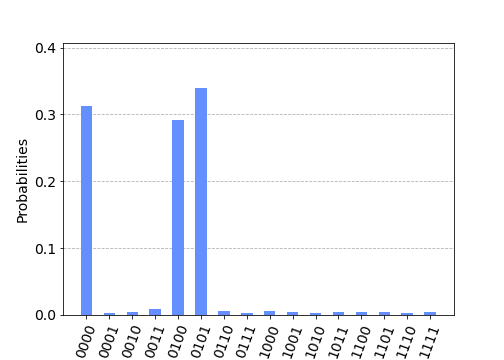
\includegraphics[width=0.7\textwidth]{assets/16x16-simulation.png}
    \caption{Probability of measuring the row-index $j$ after running the QVMP
    oracle}
    \label{fig:qvmp_oracle_sample_execution}
  \end{figure}
\end{frame}

% TODO insert circuit metrics
% TODO insert transpilation and simulation times

\begin{frame}[t,fragile]{Future work}
  \begin{exampleblock}{Automated synthesis of oracles}
    Extend existing work on reversible compilers to support higher-level
    programming constructs like lists, records, multi-dimensional arrays
  \end{exampleblock}
  \begin{itemize}
    \item Encoding classical decision functions into quantum circuits is
      error-prone and cumbersome
    \item Previous work (REVS, Quipper) have shown that we can automate
      classical to reversible compilation
  \end{itemize}
  \begin{lstlisting}[frame=single,language=ML, numbers=left]
(* Example program describing the QVMP oracle *)

[@@oracle]
let find_row_mismatch a y z =
  find_idx (fun idx value -> value <> z[idx]) (a * y)
  \end{lstlisting}
\end{frame}

\begin{frame}[t]{Future work (contd)}
  \begin{exampleblock}{Better encoding of matrices}
    Investigate more efficient encodings of matrices and related operations
  \end{exampleblock}

  \begin{itemize}
    \item $n$-qubit quantum system can encode a total of $2^n$ states
    \item QROM is still linear in space complexity
    \item Alternative approach encodes the entries of the matrix as amplitudes
      of the quantum system but is harder to work with
  \end{itemize}
\end{frame}

\begin{frame}[t]{Future work (contd)}
  \begin{exampleblock}{Transpilation time bottlenecks}
    Investigate bottle-necks in transpilation
  \end{exampleblock}
  \begin{itemize}
    \item Transpilation becomes exponentially slow as the number of qubits
      increases
    \item Makes it harder to scale and test circuit implementations
    \item Cursory investigation into Qiskit's transpile method revealed that
      SWAPs may be the bottleneck
  \end{itemize}
\end{frame}

\begin{frame}{End of talk}
  \begin{centering}
    Questions?
  \end{centering}
\end{frame}

\end{document}
